\documentclass[10pt,a4paper]{article}
\usepackage[margin=0.81in]{geometry}
\usepackage[T1]{fontenc}
\usepackage[utf8]{inputenc}
\usepackage{lmodern,microtype,graphicx,amsmath,amssymb,booktabs,tabularx,array,float,xcolor,hyperref}
\hypersetup{colorlinks=true,urlcolor=blue!45!black,linkcolor=black,citecolor=blue!45!black}
\setlength{\parskip}{4pt}\setlength{\parindent}{12pt}
\graphicspath{{../figures/}}
\title{Constraint-Valid Tool Selection Under Description Variation\\\large A Reproducible Study with Lexical Retrieval and Metadata Filtering}
\author{Sagnik Dutta\\\small Indian Institute of Information Technology, Allahabad\\\small M.Tech. in IT, Cyber Laws and Information Security}
\date{November 2026}
\begin{document}
\maketitle
\begin{abstract}
Choosing an API that matches the subject of a user request does not guarantee that it can complete the requested operation. A weather service, for instance, may cover the right region but return historical data when a live feed is needed. We investigate this distinction using a deliberately small, transparent tool-selection benchmark. A deterministic generator produces 96 API descriptions and a test set of 228 requests, including 192 feasible selections, 24 requests with unavailable output formats and 12 tasks requiring no external call. Two lexical retrievers are compared with a metadata-aware selector and two filter ablations under three descriptions of the same tool catalog. On the original descriptions, word-level TF--IDF correctly handles 112/228 requests (49.12\%), character-level TF--IDF handles 128/228 (56.14\%) and the constraint-aware rule system handles 228/228 (100\%). Removing the domain or output-format filter reduces the latter to 64.91\% and 89.47\%, respectively. All values were generated by the supplied scripts. This apparent advantage is tightly bounded: the rules have explicit access to the same ontology used to generate the labels, and the lexical methods cannot abstain. The experiment therefore provides an auditable demonstration of evaluation design and its confounds, not evidence about the performance of language-model agents in real deployments.
\end{abstract}
\noindent\textbf{Keywords:} tool retrieval, constraint validity, function calling, abstention, synthetic evaluation, ablation study.
\section{Introduction}
The correct tool is not always the tool whose description sounds most like the user's question. A request for live information in India may be incompatible with an otherwise relevant historical or global service. Tool-using language models must eventually confront these details when the number of available APIs grows. Their performance can suffer even when the selected API is fluent in its name and valid in its syntax.

The literature documents several related challenges. Gorilla investigates API invocation amid changing documentation~\cite{patil2023gorilla}, and ToolLLM connects retrieval with large-scale tool use~\cite{qin2024toolllm}. ToolSandbox and $\tau$-bench examine interactions in which the choice of action depends on state and user feedback~\cite{lu2025toolsandbox,yao2024taubench}. Tool descriptions have also been shown to influence selection behavior, while more recent research studies redundancy and tool-selection bias~\cite{faghih2025toolpreferences,blankenstein2026biasbusters,liu2026toolscope}. These studies motivate careful evaluation of the initial tool-selection decision, but the present work does not reproduce their models or claim a new general-purpose selection algorithm.

We instead ask what can be established in a controlled static environment. Specifically, can simple lexical matching distinguish tools that share a subject area but differ in operational metadata? How much of an observed improvement can be attributed to enforcing binding constraints? And do superficial changes to documentation affect the outputs? These questions are narrow enough to answer with a transparent benchmark, without making undocumented claims about production systems.

The study is a controlled comparative investigation. Its deliverables are the task generator, complete cases and tool catalog, runnable selectors, raw per-case outputs, aggregation scripts, a description-stress test, filter ablations and a complete execution record. Its main limitation is equally important: the same explicit attributes used to produce gold labels are available to the rule-based selector. The resulting score is a ceiling effect under a favorable representation, not proof of semantic understanding.

\section{Related work and study boundary}
\subsection{From API retrieval to tool-use benchmarks}
ToolLLM makes API retrieval a practical stage of working with a large catalog~\cite{qin2024toolllm}. Gorilla investigates accurate API calls and adapting to changing documentation~\cite{patil2023gorilla}. Neither reported system is actually reproduced in this experiment. Our lexical baselines are simpler, independently implemented comparators with a common task format. They represent retrieval behavior rather than a full model-based tool-calling policy.

Evaluations with richer environments address different questions. ToolSandbox uses stateful and conversational interactions, while $\tau$-bench measures agent reliability across repeated tool-user exchanges~\cite{lu2025toolsandbox,yao2024taubench}. The static requests here do not require execution, parameter construction, recovery or sequential planning; correctness is defined only over the first selected capability or justified abstention.

\subsection{Description quality and tool redundancy}
Faghih et al. report that relatively small changes to a tool's description can affect the preferences of language-model agents~\cite{faghih2025toolpreferences}. BiasBusters and ToolScope provide related evidence that selection across equivalent or redundant candidates is sensitive to metadata and filtering design~\cite{blankenstein2026biasbusters,liu2026toolscope}. These findings rule out a blanket novelty claim that ``description sensitivity'' was previously unstudied. Our narrower question is what happens under a fixed, explicitly constrained catalog when the retrieval method is changed and operational filters are ablated.

\section{Research questions}
\textbf{RQ1:} Under a shared catalog, how do word and character TF--IDF retrieval compare with deterministic metadata filtering on tool-selection validity?

\textbf{RQ2:} What is the effect of removing domain and output-format checks from the constrained selector?

\textbf{RQ3:} Does description field order or appended generic promotional text change test-set decisions while the advertised capabilities remain fixed?

All three questions are evaluated descriptively. We do not infer a general causal effect on a population of LLM agents. Any apparent improvement must be interpreted together with the additional structured information available to the rule-based system.

\section{Benchmark construction}
\subsection{Catalog and query cases}
The generator defines twelve service domains: weather, currency, maps, news, translation, stocks, sports, flights, traffic, hotels, shopping and health-related facility lookup. Each is combined with two regions (India or global), two freshness labels (live or historical) and two formats (JSON or CSV). The Cartesian product gives $12\times2\times2\times2=96$ tools.

Each generated tool has an identifier, the four metadata fields and a textual description. The case generator produces three sets of requests from disjoint \emph{template strings}: train, development and test. This is a language-template separation, not a separation of conceptual domains or catalog vocabulary. There is no learned model training step; the split names exist to expose reproducibility and lexical variation. Test cases reuse all twelve domains and the same finite ontology as the earlier partitions.

Of 228 held-out test requests, 192 have exactly one valid catalog entry, 24 request an unsupported XML or YAML format and 12 explicitly ask for a definition without using an external tool. The last two conditions are both scored as abstention but are distinguished in the saved case metadata. This matters because the reasons for not acting are different. No external user records, live service calls or proprietary data enter the benchmark.

\subsection{Labeling protocol}
For feasible cases, a gold tool is the unique catalog entry matching domain, coverage, freshness and format. For unavailable-format cases and no-tool cases, the correct decision is $\bot$. The gold mapping is mechanically generated from the same metadata schema as the catalog. This makes label consistency easy to test but creates an important dependence: a selector that understands these literal fields is likely to achieve very high accuracy by design. No independent human adjudication or naturally occurring user-query corpus is claimed.

\section{Methods}
\subsection{Retrieval baselines}
The first comparator uses scikit-learn's \texttt{TfidfVectorizer} with word unigrams and bigrams, followed by cosine similarity between a user request and each tool description. The second uses character n-grams of lengths three through five. Both return the highest scoring tool, with deterministic tool-ID tie-breaking. Neither comparator has an abstention mechanism. This is a relevant architectural difference that must be accounted for when comparing the overall metric.

\subsection{Constraint-aware selection and ablations}
The constraint-aware system reads explicit terms for domain, region, freshness and output format from the request, filters the tool inventory to records that match, and then applies word-level TF--IDF ranking among the survivors. If no entry remains, it returns $\bot$. Requests that explicitly prohibit an external tool call are also mapped to abstention. The method is a hand-designed rule system; it is not a learned semantic parser.

Two ablations each remove one filtering step while retaining the rest of the implementation. The ``without domain'' variant permits unrelated categories to compete; the ``without format'' variant ignores requested output type. In both cases the remaining checks still operate. These ablations identify how much these specific checks contribute on the generated test cases. They do not demonstrate that the same checks would solve free-form requests.

\subsection{Description conditions}
Three catalog presentations are considered. The \emph{original} presentation uses the generated service descriptions. The \emph{reordered} presentation changes the order in which format, freshness, coverage and domain phrases appear, without changing their values. The \emph{distractor} presentation appends a generic positive sentence to descriptions. These are controlled text perturbations, not a representation of adversarial attacks against deployed agents.

\section{Evaluation protocol and implementation}
For request $i$, let $G_i$ be the set of valid tool IDs. The selector predicts $\hat{t}_i\in T\cup\{\bot\}$. The binary score is
\begin{equation}
 s_i=\begin{cases}
  1, & G_i\ne\emptyset\;\text{and}\;\hat{t}_i\in G_i,\\
  1, & G_i=\emptyset\;\text{and}\;\hat{t}_i=\bot,\\
  0, & \text{otherwise.}
 \end{cases}
\qquad A=\frac{1}{N}\sum_i s_i.
\end{equation}

The program records the case ID, split, condition, catalog variant, method, prediction, gold set, correctness indicator and elapsed time for each selection. Identical generated inputs are used for all methods. Files in \texttt{results/} preserve per-case predictions and aggregated results; \texttt{results/environment.json} saves Python package versions, random seed and dataset hashes. Eight unit tests cover catalog consistency, case counts, abstention examples, known-valid behavior, determinism, description metadata preservation and a bootstrap sanity check.

For each paired method comparison, 3,000 bootstrap resamples over test-case IDs yield a descriptive interval for the difference in accuracy. Because examples share domains and templates, these resamples must not be interpreted as independent samples from natural user behavior. Per-request latency is logged but is not subjected to a controlled timing study and is not used to claim relative efficiency.

\section{Results}
\begin{table}[H]
\centering\small
\caption{Actual original-description test results (228 cases).}\label{tab:results}
\begin{tabular}{@{}lrr@{}}\toprule
Selector & Correct / 228 & Accuracy\\\midrule
Word TF--IDF &112&49.12\%\\
Character TF--IDF&128&56.14\%\\
Constraint-aware&228&100.00\%\\
Constraint-aware without domain filter&148&64.91\%\\
Constraint-aware without format filter&204&89.47\%\\\bottomrule
\end{tabular}
\end{table}

Table~\ref{tab:results} is computed directly from the test rows saved in \texttt{results/metrics.csv}. Among the 192 feasible requests, word and character TF--IDF obtain 58.33\% and 66.67\%, respectively. They cannot abstain on the 24 impossible-format and 12 no-tool cases, so both achieve zero on those subsets. The constraint-aware system handles each of the 228 generated cases correctly. Its performance is unsurprising once the label generator and filtering rules are read together.

\begin{figure}[H]\centering
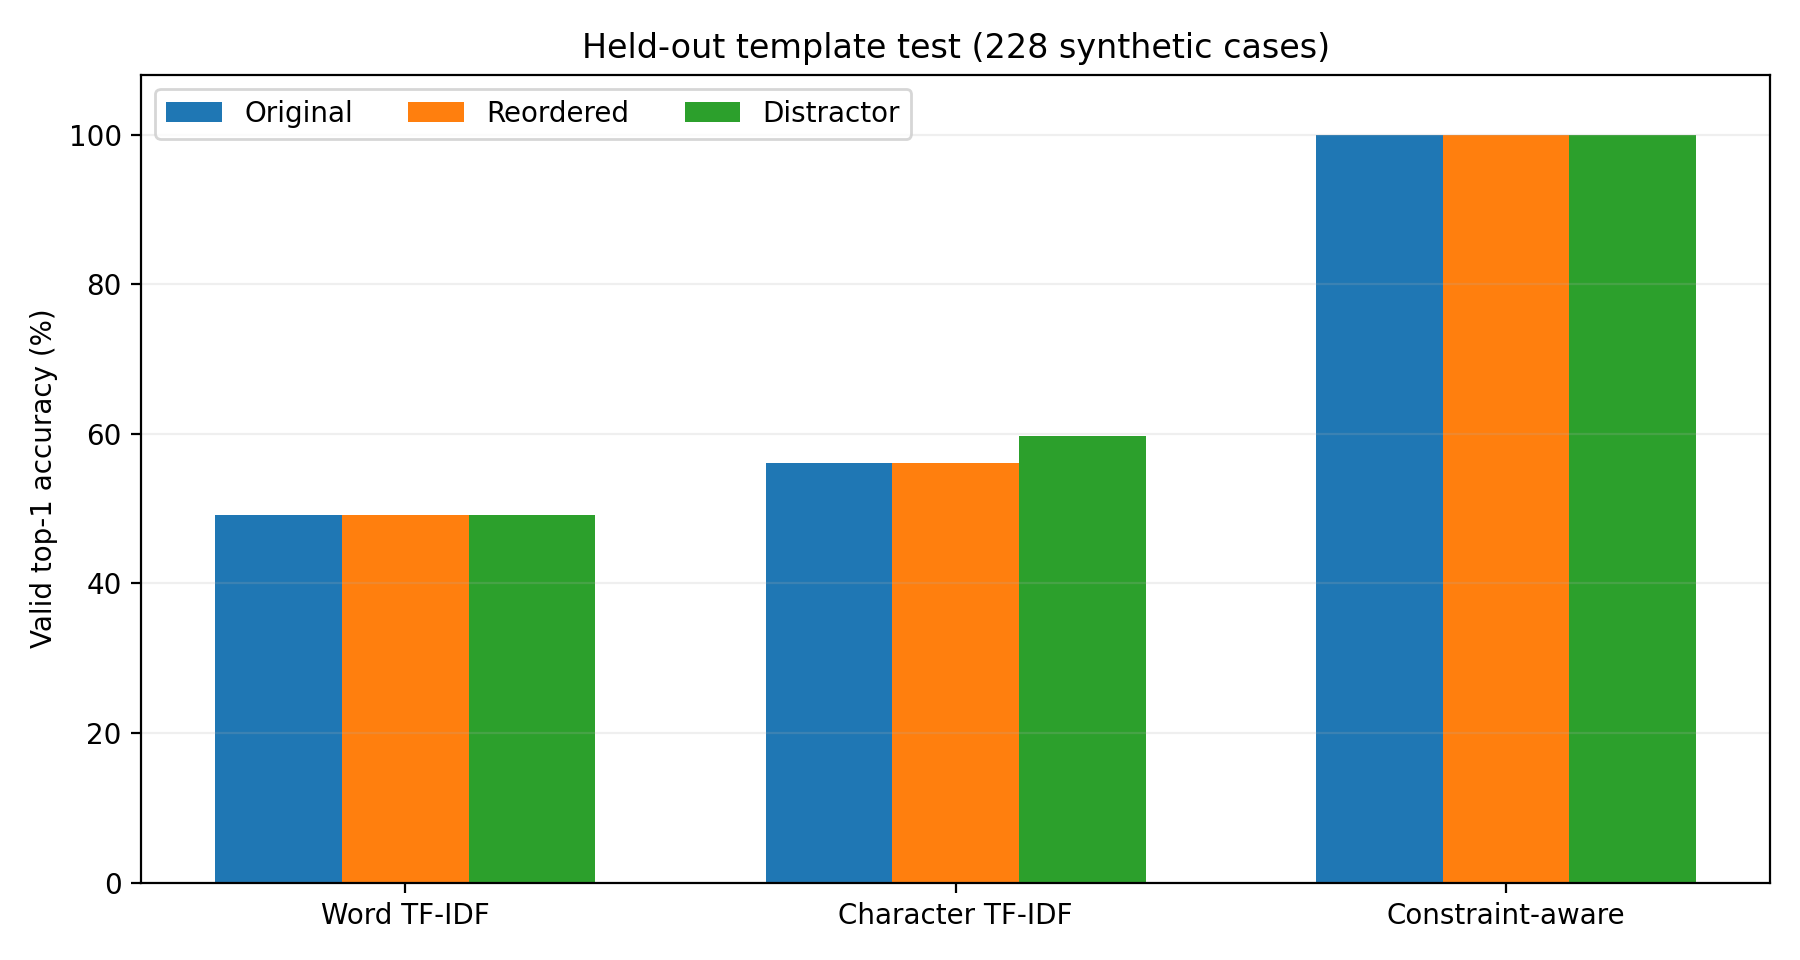
\includegraphics[width=.94\linewidth]{accuracy.png}
\caption{Test-set accuracy for five methods under original, reordered and distractor description conditions. Generated by the repository's plotting script.}\label{fig:accuracy}
\end{figure}

The paired accuracy difference between constraint-aware selection and word TF--IDF on original descriptions is $50.88$ percentage points. The per-item bootstrap 95\% interval is $[44.30,57.46]$ percentage points (as rounded from saved results). This interval describes the variability across resampled synthetic items only. It is not evidence of statistical generalization to real-world tool catalogs.

\begin{figure}[H]\centering
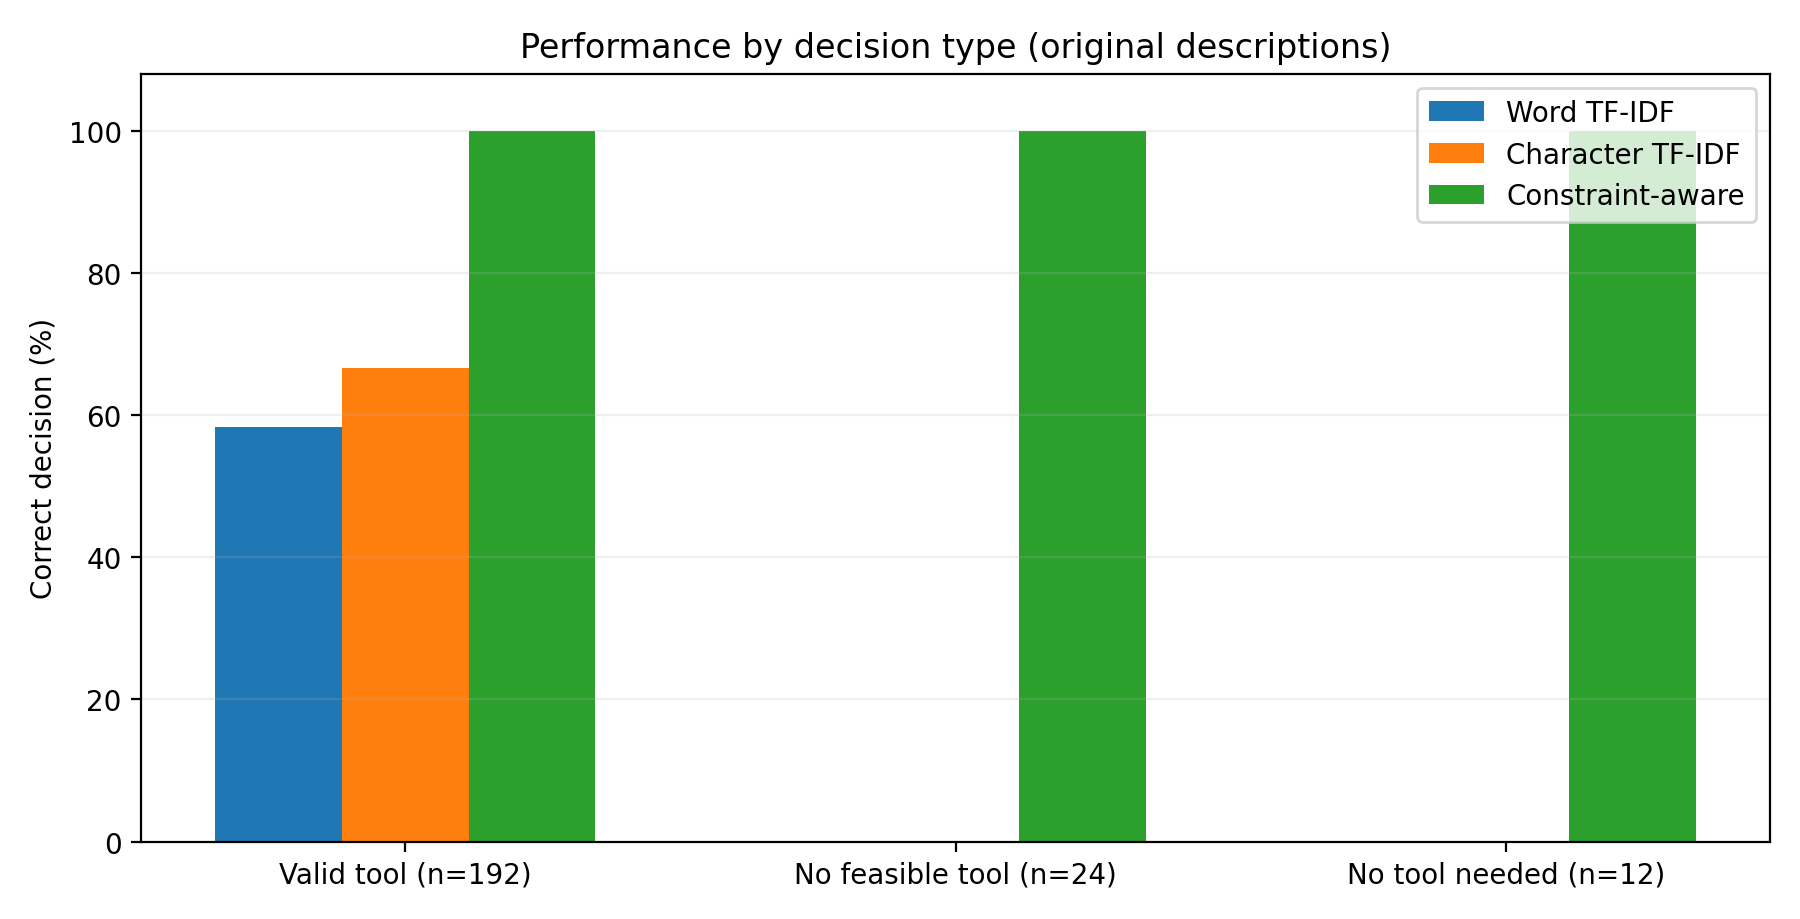
\includegraphics[width=.92\linewidth]{error_categories.png}
\caption{Performance by test-case condition under original descriptions; the distinction between available-tool and abstention cases is explicit.}\label{fig:errors}
\end{figure}

Description field reordering does not change the aggregate test accuracies in this implementation. The appended generic sentence changes some character-level retrieval outcomes but not the constraint-aware total. These results should not be read as a universal claim of robustness to document changes, especially because the perturbations preserve exact capability labels.


\section{Diagnostic breakdown of observed errors}
The aggregate metric conceals two different kinds of failure: selecting a tool with the wrong attributes and selecting a tool when no appropriate external action exists. Table~\ref{tab:cases} separates these outcomes using the original catalog description. This breakdown is computed from the same saved results as Table~\ref{tab:results}; no additional experiment is implied.

\begin{table}[H]\centering\small
\caption{Correct decisions by test-case type, original descriptions.}\label{tab:cases}
\begin{tabular}{@{}lrrr@{}}\toprule
Method & Feasible (192) & No valid (24) & No tool (12)\\\midrule
Word TF--IDF&112&0&0\\
Character TF--IDF&128&0&0\\
Constraint-aware&192&24&12\\
Without domain&112&24&12\\
Without format&192&0&12\\\bottomrule
\end{tabular}
\end{table}

This table changes the interpretation of the ablations. Removing the domain check leaves the negative-case handling intact; it mainly affects the choice among tools when a feasible tool exists. The no-domain version selects the correct tool on 112 of the 192 feasible requests, exactly the same count as the word-level lexical method. It still returns abstention for the 36 cases that call for no tool. In contrast, removing format filtering does not harm the 192 feasible cases in this test set, but it fails every example that requests XML or YAML, because the remaining metadata checks leave JSON or CSV tools that sound relevant. The two errors therefore arise from different parts of the decision process.

A second observation concerns the two lexical baselines. Character n-grams improve the number of correct feasible choices by sixteen cases, from 112 to 128, even without any access to structured constraint fields. This is a consistent descriptive difference within the generated cases; it does not establish that character vectors are generally better retrievers. Both retrieval variants still fail the abstention cases by construction. A fairer system-level comparison would add a rejection threshold to each retrieval baseline and choose that threshold on a separate development set, rather than adding it only after seeing test outcomes.

These analyses illustrate why tool-selection accuracy should be accompanied by error categories and method capabilities. A single aggregate score cannot indicate whether a system misunderstands the target domain, ignores a binding output requirement or never learned to refrain from acting.

\subsection{What the description changes do and do not test}
The field-reordering condition preserves all the labels required by the rule selector. It is therefore a test of sensitivity to text ordering, not an evaluation of schema updates. Similarly, the generic promotional sentence introduces additional language without contradicting any operational field. The constrained policy is intentionally insensitive to that sentence because it reads only specific tokens for region, freshness, domain and format. This is a strength only in a narrow setting: if descriptions contained conflicting or partially missing capability statements, the rule system would need a defined policy for which source of information to trust.

The saved predictions make it possible to inspect changes at the case level, not just changes in aggregate accuracy. Two selectors can have the same total accuracy while failing on different requests. The repository retains request IDs and predicted IDs specifically so that such swaps can be detected. In future work, paired error-set comparisons and independently written request paraphrases would supply a stronger test of description robustness than adding generic promotional language.

\section{Discussion and threats to validity}
The experiment answers its narrow question: when every test request uses visible labels from a fixed ontology, hard filtering is an effective way to avoid selecting a tool with mismatched metadata. The ablations further show that domain and format checks matter even inside this simplified setting. However, several design choices favor the constraint-aware selector over the lexical comparisons.

First, the rule system reads precise markers drawn from the same finite set that generated the labels. It does not need to infer unstated constraints, resolve ambiguous meanings or deal with unknown capabilities. Second, the lexical baselines are required to choose some tool even when the gold action is abstention; a retrieval-plus-rejection comparator might be fairer. Third, train/development/test use different string templates but share all service categories, capability combinations and generator rules. Thus the test does not measure domain-level out-of-distribution generalization. Fourth, all feasible cases have one correct tool, whereas actual environments may have several semantically equivalent APIs.

These limitations explain why the 100\% value is not an estimate of general tool-selection competence. It is a property of a particular generated benchmark and a matching deterministic policy. Similarly, an item-level bootstrap cannot remove the dependence created by templates. A rigorous follow-on study would require independent query formulation, adjudicated validity labels, equivalent abstention capabilities for comparators and, eventually, evaluation with an actual language-model tool selector.

\section{Reproduction and conclusion}
The implementation is self-contained. The main scripts generate the catalog and cases, evaluate all five methods on three catalog presentations and save predictions, summary metrics and figures. The documented commands are:
\begin{verbatim}
python -m unittest discover -s tests -v
python -m src.run_experiment
python -m src.plot_results
python -m scripts.demo
\end{verbatim}
The accompanying repository also contains the actual execution logs and environment metadata. The study does not use a live API, trained agent or proprietary dataset.

The results demonstrate a useful lesson about the design of tool-selection benchmarks: if operational requirements are part of the problem, they should appear in the validity labels and the error analysis. At the same time, a comparison must acknowledge when one method has privileged access to the schema that produced those labels. This project offers a checkable baseline for investigating that distinction, while leaving claims about natural language understanding, deployed systems and published-model reproduction unresolved.

\begin{thebibliography}{99}\small
\bibitem{patil2023gorilla} S. G. Patil, T. Zhang, X. Wang, and J. E. Gonzalez, ``Gorilla: Large Language Model Connected with Massive APIs,'' \emph{NeurIPS}, 2024. \url{https://arxiv.org/abs/2305.15334}.
\bibitem{qin2024toolllm} Y. Qin et al., ``ToolLLM: Facilitating Large Language Models to Master 16000+ Real-world APIs,'' \emph{ICLR}, 2024. \url{https://arxiv.org/abs/2307.16789}.
\bibitem{lu2025toolsandbox} J. Lu et al., ``ToolSandbox: A Stateful, Conversational, Interactive Evaluation Benchmark for LLM Tool Use Capabilities,'' \emph{Findings of NAACL}, 2025. doi:10.18653/v1/2025.findings-naacl.65.
\bibitem{yao2024taubench} S. Yao et al., ``$\tau$-bench: A Benchmark for Tool-Agent-User Interaction in Real-World Domains,'' arXiv:2406.12045, 2024.
\bibitem{faghih2025toolpreferences} K. Faghih et al., ``Tool Preferences in Agentic LLMs are Unreliable,'' \emph{EMNLP}, 2025. doi:10.18653/v1/2025.emnlp-main.1060.
\bibitem{liu2026toolscope} M. M. Liu et al., ``ToolScope: Enhancing LLM Agent Tool Use through Tool Merging and Context-Aware Filtering,'' \emph{ACL}, 2026. \url{https://aclanthology.org/2026.acl-long.1573/}.
\bibitem{blankenstein2026biasbusters} T. Blankenstein et al., ``BiasBusters: Uncovering and Mitigating Tool Selection Bias in Large Language Models,'' \emph{ICLR}, 2026. \url{https://proceedings.iclr.cc/paper_files/paper/2026/hash/a79875cc0d046ce7ce65f03f3affaa9e-Abstract-Conference.html}.
\end{thebibliography}

\end{document}
